\label{sec:charakterbogen}\begin{quote}
    Ach ich darf mein Leben gar nicht für die Punkte opfern?
\end{quote}
\subsection{Allgemeine Daten}

Hierbei sei erst einmal gesagt, dass das endgültige Layout des Charakterbogens noch nicht fertig ist (und ich gerne Designs/Zeichnungen von euch darin einbaue um das Ganze aufzuhübschen \Laughey) und ihr deswegen hier nur pragmatische Darstellungen der jeweiligen Sektion seht, die nur aus semantischer Sicht so übernommen werden.

\index{Punkte}Wichtig ist, dass es diesmal \index{Punkte!Spezifisch (\SP)}spezifische (\SP{}) und \index{Punkte!Global/Magisch (\GP)}globale (\GP{}) Punkte gibt. \SP{} sind an eine Fertigkeiten-Gruppe gebunden. \SP{} können \(4:1\) in \GP{} umgewandelt und damit auch in anderen Gruppen eingesetzt werden (\GP{} sind allerdings nicht mehr Wert, die einzige Ausnahme hiervon ist die Magie\ldots).% TODO: link Magie

\paragraph{Allgemeine Metadaten}
\label{par:charMeta}\begin{sccenter}
    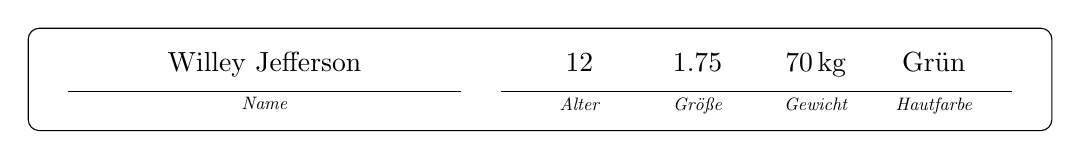
\begin{tikzpicture}[lc/.style={below,scale=0.65,font=\itshape}]
        \draw[rounded corners] (0,0) rectangle ++(13,1.3);
        \draw (0.5,0.5) -- ++(5,0) node[lc,midway] {Name} node[above,midway] {\strut{Willey Jefferson}};
        \draw (6,0.5) -- ++(6.5,0);
        \foreach[count=\i] \a/\b in {12/Alter,1.75/Größe,70\,kg/Gewicht,Grün/Hautfarbe} {
            \node[lc] at(7+1.5*\i-1.5,0.5) {\b}; 
            \node[above] at(7+1.5*\i-1.5,0.5) {\strut\a}; 
        }
    \end{tikzpicture}
\end{sccenter}
Die Daten, die dort eingetragen werden sollen, sollten ohne große Erklärung funktionieren. Deswegen hopp hopp, und weiter geht die Reise\ldots

\paragraph{Die Lebensversicherung}
\begin{wrapfigure}[4]{r}{0.375\linewidth}
    \vspace*{-0.75\topsep}\centering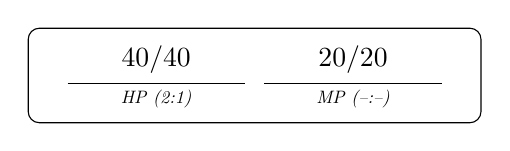
\begin{tikzpicture}[lc/.style={below,scale=0.65,font=\itshape}]
        \draw[rounded corners] (0,0) rectangle ++(5.75,1.2);
        \draw (0.5,0.5) -- ++(2.25,0) node[lc,midway] {HP (2:1)} node[above,midway] {40/{\smaller40}};
        \draw (3,0.5) -- ++(2.25,0) node[lc,midway] {MP (--:--)} node[above,midway] {20/{\smaller20}};
    \end{tikzpicture}
\end{wrapfigure}
Erstmal zu den \imp{Lebenspunkten (HP)}: 
Ihr startet mit 40, was nach verhältnismäßig wenig klingt aber schon ganz ordentlich ist im Verhältnis zum allgemeinen Schadenssystem. % TODO: LinK
Die Kosten für Leben betragen \(2:1\) und können aus allen anderen Gruppen zusammengespart werden. Der Verkaufspreis ist invertiert, ein Lebenspunkt liefert also zwei Fertigkeitenpunkte (\SP).
Die Lebenspunkte dürfen durch das verkaufen nicht auf oder unter Null gesetzt werden. Weniger Lebenspunkte werden aber auch hart bestraft\ldots

Eure Lebenspunkte sind den folgenden Regeln unterworfen:
\begin{itemize}
    \item \label{char:createNew}Fällt die Anzahl der Lebenspunkte aus einem beliebigen Grund auf oder unter \(0\) so scheidet der Charakter umgehend aus. In diesem Fall ist ein neuer Charakter zu erstellen, dessen Level zwei unter dem des bisher niedrigsten Gruppenlevels ist\footnote{Das Level kann über diese Mechanik nicht unter 1 gesetzt werden.}.
    \item Verursacht ein Angriff mindestens so viel Schaden wie die Hälfte der aktuellen Lebenspunkte, so ist eine Probe zu werfen (hier erscheint eine Referenz, sobald es diese Probe gibt). % TODO: link
    \item Fällt die Anzahl der Lebenspunkte unter 5, so gilt der Charakter als \imp{schwer verwundet} und kann eigenhändig keine Aktionen wie laufen, oder gar kämpfen durchführen.
    \item Jegliche Form von Heilung (egal ob magisch oder physisch) lässt sich für jede Wunde nur einmal pro Tag\footnote{Solche Begrenzungen setzen wir lose auf \say{alle \(24\)} Stunden, nicht das einer um Mitternacht direkt zwei Bandagen anbringen möchte.} anwenden.
    \item \index{Schlaf}Eine vom Spielmeister als \say{angenehm} eingestufte Nacht (in der geschlafen wurde) stellt \(\dice{1}{6} + 1\) Leben wieder her, sofern am Tag mindestens einmal am Tag gegessen wurde. Es steht dem Spielmeister frei, Schaden für das Unterlassen einer Nahrungsaufnahme zu verteilen.
\end{itemize}

Die \imp{Manapunkte (MP)} sind auf 20 beschränkt. Das Limit kann weder durch \SP/\GP{}, noch durch einen Levelaufstieg verändert werden.
Es existieren Gegenstände und Tier die selbst Mana innehaben und so zum wiederauffüllen verwendet werden können. Der Pool ist für den Anwender aber stets auf 20 eingegrenzt\footnote{So ist auch Magie in die beliebig viele Manapunkte investiert werden können auf maximal 20 Manapunkte beschränkt. Weitere \say{Manapunkte} können aber durch die gegebenen Regeln aufgebracht werden}. Für die Manapunkte gelten die folgenden Regeln:
\begin{itemize}
    \item Fällt das Mana, aus irgendeinem Grund, auf 0, so schließt dies nicht aus weiter Magie einzusetzen. Für je einen Lebenspunkte kann je ein weiterer Manapunkt investiert werden. So ist es auch möglich weiter zu zaubern, wenn der Mana-Pool aufgebraucht ist. Ein Magieanwender kann durch diese Mechanik zu Tode kommen.
    \item Schlaf generiert \emph{keine} Manapunkte.
    Magier können anstelle zu Schlafen auch \index{Meditation}\imp{Meditieren} und erhalten \(\dice{1}{4} + 1\) Manapunkte für eine \say{angnehme Nacht} zurück.
\end{itemize}

\paragraph{Level}
\begin{wrapfigure}[4]{r}{0.375\linewidth}
    \vspace*{-0.75\topsep}\centering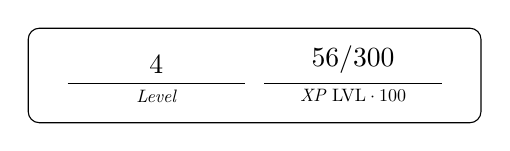
\begin{tikzpicture}[lc/.style={below,scale=0.65,font=\itshape}]
        \draw[rounded corners] (0,0) rectangle ++(5.75,1.2);
        \draw (0.5,0.5) -- ++(2.25,0) node[lc,midway] {Level} node[above,midway] {4};
        \draw (3,0.5) -- ++(2.25,0) node[lc,midway] {XP \(\mathrm{LVL} \cdot 100\)} node[above,midway] {56/{\smaller300}};
    \end{tikzpicture}
\end{wrapfigure}
Ein Charakter startet auf \imp{Level (LVL)} 1, sofern er nicht durch die \say{\link[char:createNew]{Neuerstellungsmechanik}} auf einem höheren Level beginnt.
Die \imp{Erfahrungspunkte (XP)} beginnen in jedem Falle bei \(0\).
Um ein Level aufzusteigen werden jeweils \(\mathrm{LVL} \cdot 100\) Erfahrungspunkte benötigt.
Um von Level 1 auf Level 2 aufzusteigen werden also 100, um von Level 2 auf Level 3 aufzusteigen werden 200 Erfahrungspunkte benötigt, und so weiter\ldots

Für den \imp{Levelaufstieg} von Level 1 auf Level 2 werden \SP[6] pro Kategorie und \GP[3] vergeben.
Jeder Aufstieg darüber wird mit \SP[6] in jeder Kategorie und \GP[4] vergütet.

\subsection{Ausrüstung}

Zusätzlich zu eurem super duper gezeichneten \imp{Bild} des Charakters\footnote{An das Bild ist eine hohe Erwartungshaltung gerichtet ist, schließlich soll das Verlieren eines charakters ja auch richtig weh tun \Winkey.} geht es nun einmal um die \imp{Ausrüstung} welches sein Antlitz teils überdeckt.
Auch wenn es hier etliche Segmente gibt, braucht ihr nicht für jede ein eigenes Rüstungsteil. Ihr könnt euch die \say{Deko}-Kleidung aussuchen. Diese Kleidung hat aber
keine Werte (ist also wirklich nur kosmetischer Natur) und hilft auch in Debatten wie \say{Aber schau mal auf dem Bild trägt der eindeutig ein Jetpack} nicht weiter.
Jeder der folgenden Slots kann mit einem Element/Kleidungsstück belegt werden welches
Rüstungspunkte und sogar weitere Vorteile mit sich bringen mag. Solche Gegenstände gilt
es grundlegend zu erwerben. % TODO: link shopping
\begin{description}
    \item[Gesicht:] Platz für Masken, Sonnenbrillen, \ldots{} Dieser Slot kann (so dem Willen des Spielleiters) auch diverse Gegenstände fassen.
    \item[Kopfbedeckung:] Helme, Hüte, Perücke, \ldots{} Auch dieser Slot kann diverse Gegenstände fassen.
    \item[Mantel:] Jacken, Mäntel, Capes, \ldots{} Wird hier beispielsweise ein Wintermantel für die Kälte getragen kann dies am Tag für Nachteile sorgen. Solche Gegenstände können dann natürlich im Inventar verstaut werden.
    \item[Oberkörper:] Hemd, Bluse, Rüstung, \ldots{}
    \item[Hüfte:] Köcher, Wurfmesser, Munition \ldots{} Es kann auch als \say{Quick-Recharge-Slot} betrachtet werden. Im Kampf legt schließlich keiner den Rucksack auf dem Boden und sucht nach Munition.
    \item[Handschuhe:] Krallen, Handschuhe, \ldots{}
    \item[Beine:] Lange- und Kurze-Hose, Rock, \ldots{}
    \item[Füße:] Schuhwerk. Hier haben auch kosmetische Schuhe eine Wirkung. Keine Sohle und heißer Sand ist jetzt nicht die erfreulichste Kombination.
\end{description}

Doch wohin gehören nun meine Waffen und die ganzen Schildkrötenkuscheltiere? Für diese gibt es separate Slots.
% Getragene Waffe und Schnellzugriffe...

\subsection{Inventar}

\subsection{Fertigkeiten}